\documentclass[dvipdfmx]{ujarticle}
\usepackage[dvipdfmx]{graphicx}
\usepackage{here}
%% 高さの設定
\setlength{\textheight}{\paperheight}   % ひとまず紙面を本文領域に
\setlength{\topmargin}{-5.4mm}      % 上の余白を20mm(=1inch-5.4mm)に
\addtolength{\topmargin}{-\headheight}  % 
\addtolength{\topmargin}{-\headsep}     % ヘッダの分だけ本文領域を移動させる
\addtolength{\textheight}{-50mm}    % 下の余白も20mmに
%% 幅の設定
\setlength{\textwidth}{\paperwidth}     % ひとまず紙面を本文領域に
\setlength{\oddsidemargin}{-5.4mm}  % 左の余白を20mm(=1inch-5.4mm)に
\setlength{\evensidemargin}{-5.4mm} % 
\addtolength{\textwidth}{-40mm}     % 右の余白も20mmに
\pagestyle{empty}   %ページ番号なし

\newcommand{\g}[1]{\boldsymbol{#1}}
\newcommand{\lw}[1]{\smash{\lower2.0ex\hbox{#1}}}
\renewcommand{\baselinestretch}{1.0}

\makeatletter
\def\mojiparline#1{
    \newcounter{mpl}
    \setcounter{mpl}{#1}
    \@tempdima=\linewidth
    \advance\@tempdima by-\value{mpl}zw
    \addtocounter{mpl}{-1}
    \divide\@tempdima by \value{mpl}
    \advance\kanjiskip by\@tempdima
    \advance\parindent by\@tempdima
}
\def\linesparpage#1{
    \baselineskip=\textheight
    \divide\baselineskip by #1
}

\title{単一QD-SOAを用いた全光XOR-AND回路}
\author{4616072 畑洋樹}

\begin{document}
\mojiparline{43}
\maketitle

\section{はじめに}
近年のインターネット通信端末の増加と普及により,光通信による通信の高速化と大容量化が必要不可欠となっている.
現在の光通信では,信号処理を行う際に一度光信号から電気信号へと変換するため通信速度の最大値が電気信号の処理速度に依存してしまうという課題がある.
従って電気信号への変換処理が必要ない全光信号処理技術を構成する全光論理回路の研究が進められているが,従来研究として実装されている全光論理回路の多くは光がデバイスに入射した際に発生する非線形光学効果を利用している.
その中でも量子ドット半導体光増幅器(Quantum-Dot Semiconductor Optical Amplifiers: QD-SOA)を用いた全光論理回路が提案されている.
QD-SOAは量子ドット構造の活性層を持つ光増幅器のことであり,電子を量子ドット内に閉じ込めることで従来の光増幅器よりも大きな利得を得ることができる.
従来研究として提案されている全光XOR回路ではマッハ・ツェエンダー干渉系(Mach-Zehnder Interferometer:MZI)を用いた回路が提案されている.
しかし,MZIを用いた全光回路は同一特性のQD-SOAを2つ使用しなければならないが同一特性のQD-SOAを製造することは非常に困難という問題がある.
上記の問題点を踏まえ、かつ特定の波長の光を取り出すデバイスであるOptical Fileter(OF)の波長を変更することで出力としてXOR回路としてだけでなくAND回路としても使用できる.

\section{単一QD-SOAを用いた全光XOR-AND回路}

\begin{figure}[H]
  \begin{center}
    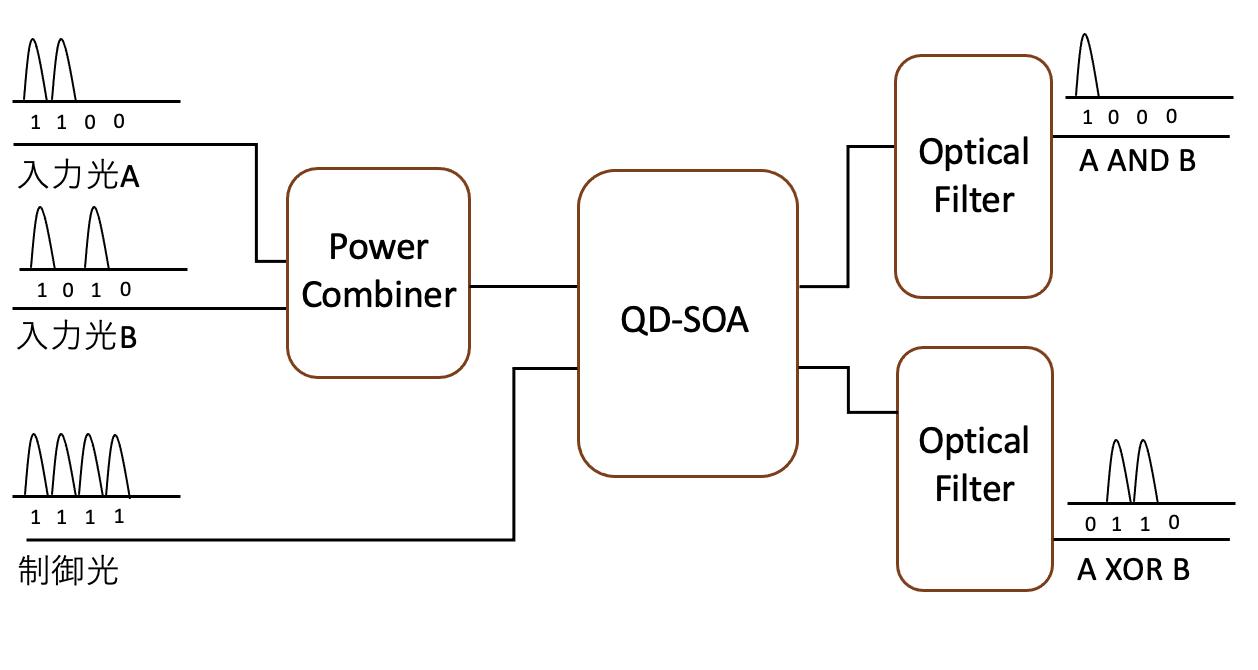
\includegraphics[width=15cm]{images/kairo2.png}
    \caption{提案する全光XOR-AND回路の構成}
  \end{center}
\end{figure}
提案する全光回路ではまず, 入力光A,Bを複数の光を合波するデバイスであるPowerCombiner(PC)に入射させる.
その後合波された光と制御光を入力としたQD-SOAで光を増幅させ,最後に特定の波長の光を取り出すデバイスであるOptical Filter(OF)から基本論理回路として必要な波長のみを取り出し最終的な出力光とする.

\section{シミュレーション}
\subsection{条件及び評価指標}
本研究では OptiSystem16.1.0, MATLAB 2019a を用いてシミュレーションを行った.
QD-SOAは光の伝搬方程式, キャリアのレート方程式及び伝達行列法(Transfer Matrix Method:TMM)を用いてシミュレーションを行った.ビットレートは160Gbpsとした.
光の伝搬方程式はQD-SOA内の光電界に関する式であり,キャリアのレート方程式はQD-SOA内の時間変化によるキャリアの変化を表す式である.
また,伝達行列法はQD-SOAを光の伝搬方向に対して細かく分割しキャリア密度, 光子密度, 利得を繰り返し求めることで結果的に出力される光電界を求める手法である.
今回シミュレーションで使用するパラメータは表1[1]に示したものを用いた.\\
 シミュレーションでは入力光強度と各演算に対応する光フィルタの指定波長を変化させ、それぞれの条件に対する消光比が最も高くなるようなパラメータ探索を行う.
なお,各演算に対応する光フィルタの指定波長はスペクトラムの広がりから指定する.

\begin{table}[H]
  \caption{シミュレーションで用いるパラメータ}
  \centering
    \begin{tabular}{ccc}
      \hline
      パラメータ名 & 値 & 単位 \\
      \hline
      QD-SOAの長さ & $ 3.0 \times 10^{-3} $ & $m$\\
      QD-SOAの厚さ & $ 0.25 \times 10^{-6} $ & $m$\\
      QD-SOAの幅 & $ 3.0 \times 10^{-6} $ & $m$\\
      量子ドット密度 & $ 5.0 \times 10^{14} $ & $m^{-2}$\\
      キャリア寿命(WL→ES) & $ 3.0 \times 10^{-12} $ & $s$ \\
      キャリア寿命(ES→WL) & $ 1.0 \times 10^{-9} $ & $s$\\
      キャリア寿命(WL→系外) & $ 2.0 \times 10^{-9} $ & $s$\\
      キャリア寿命(ES→GS) & $ 0.16 \times 10^{-12} $ & $s$\\
      キャリア寿命(GS→ES) & $ 1.2 \times 1o^{-12} $ & $s$\\
      キャリア寿命(GS→系外) & $ 0.4 \times 10^{-9} $ & $s$\\
      注入電流 & $5.0 \times 10^{-2}  $ & $A$\\
      最大利得 & $12.0 $ & $cm^{-1}$\\
      損失係数 & $2.0$ & $cm^{-1}$\\

      \hline

    \end{tabular}
\end{table}

\subsection{評価指標}
評価指標としてアイダイアグラム(eye diagram)および消光比(Extinction Ratio: ER)を用いる.
アイダイアグラムとは信号光を1ビット幅間隔で分割し,重ね合わせて描画したグラフのことであり,
消光比は ${P^1}_{min}$を "1" として出力された光の中で最も強度が弱いときの光強度の値,
${P^0}_{min}$を "0" として出力された光の中で最も強度が強い時の光強度の値としたときに
$ER[dB] = 10 \log{10}{\frac{{P^1}_{min}}{{P^0}_{max}}}$ で算出される指標である.
この値が大きいほど出力光が "0" , "1" の区別がつきやすい優れた波形であることを示す.

\subsection{光フィルタの波長選択}
入力光の値によるQD-SOAからの出力スペクトラムを下記に示す. \\
光フィルタを用いて実践で囲った波長を分離するとXOR演算として機能し, 破線で囲った波長を分離するとAND演算として機能する.

\begin{figure}[H]
  \begin{tabular}{cc}
    \begin{minipage}[t]{0.45\hsize}
      \centering
      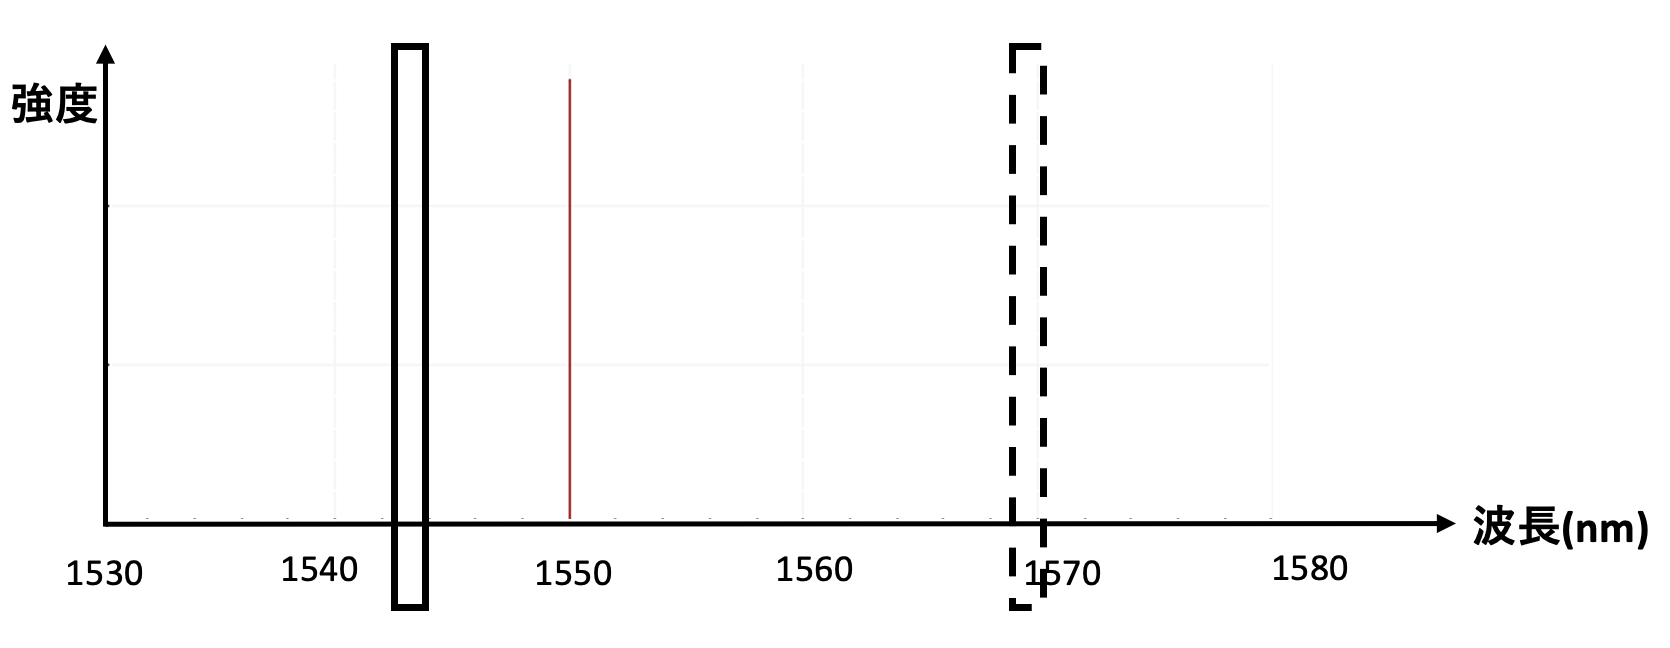
\includegraphics[width=7cm]{images/00_spectrum.png}
      \caption{入力光A=0, 入力光B=0の場合のスペクトラム}
    \end{minipage} &
    \begin{minipage}[t]{0.45\hsize}
      \centering
      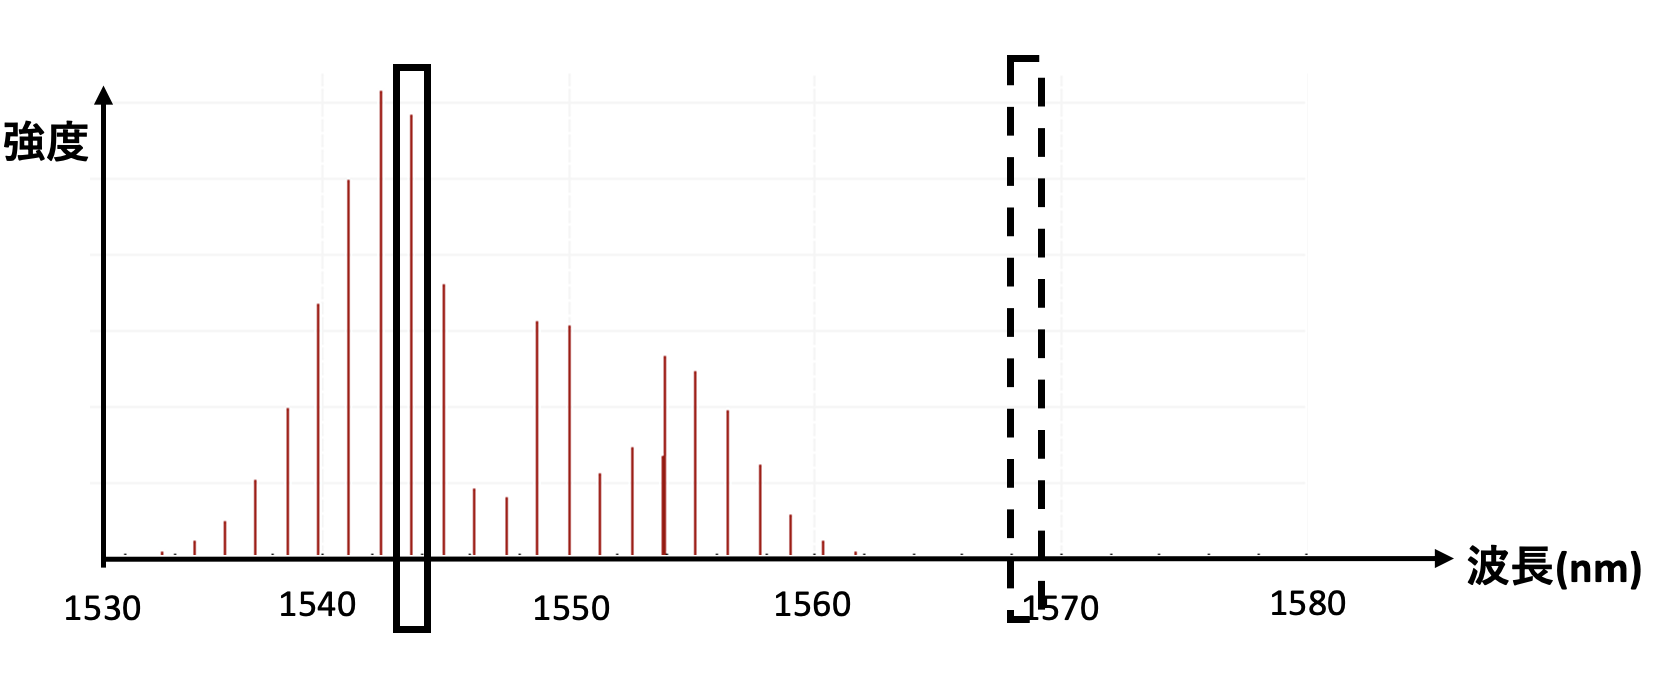
\includegraphics[width=7cm]{images/01_spectrum.png}
      \caption{入力光A=1, 入力光B=0の場合のスペクトラム}
    \end{minipage}
    \\
    \begin{minipage}[t]{0.45\hsize}
      \centering
      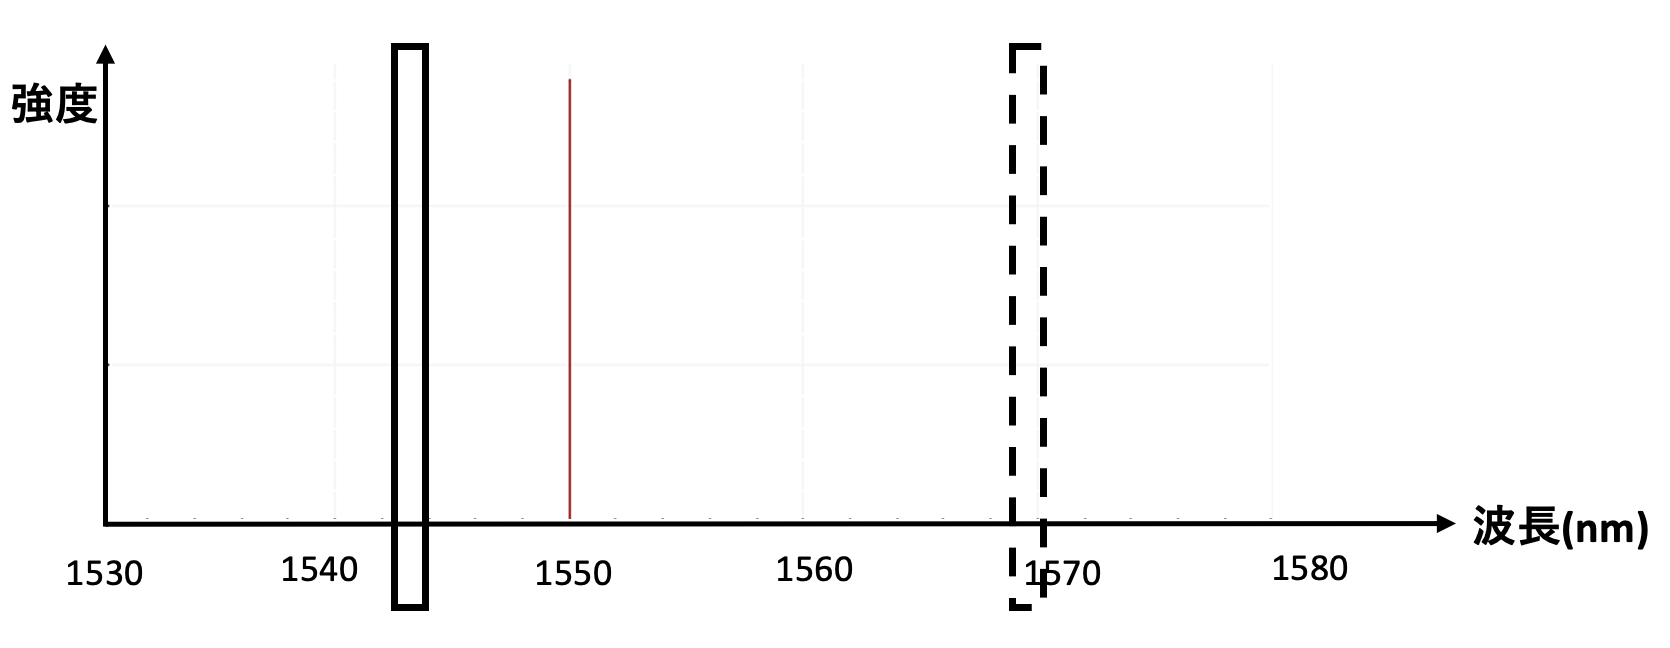
\includegraphics[width=7cm]{images/00_spectrum.png}
      \caption{入力光A=0, 入力光B=1の場合のスペクトラム}
    \end{minipage} &
    \begin{minipage}[t]{0.45\hsize}
      \centering
      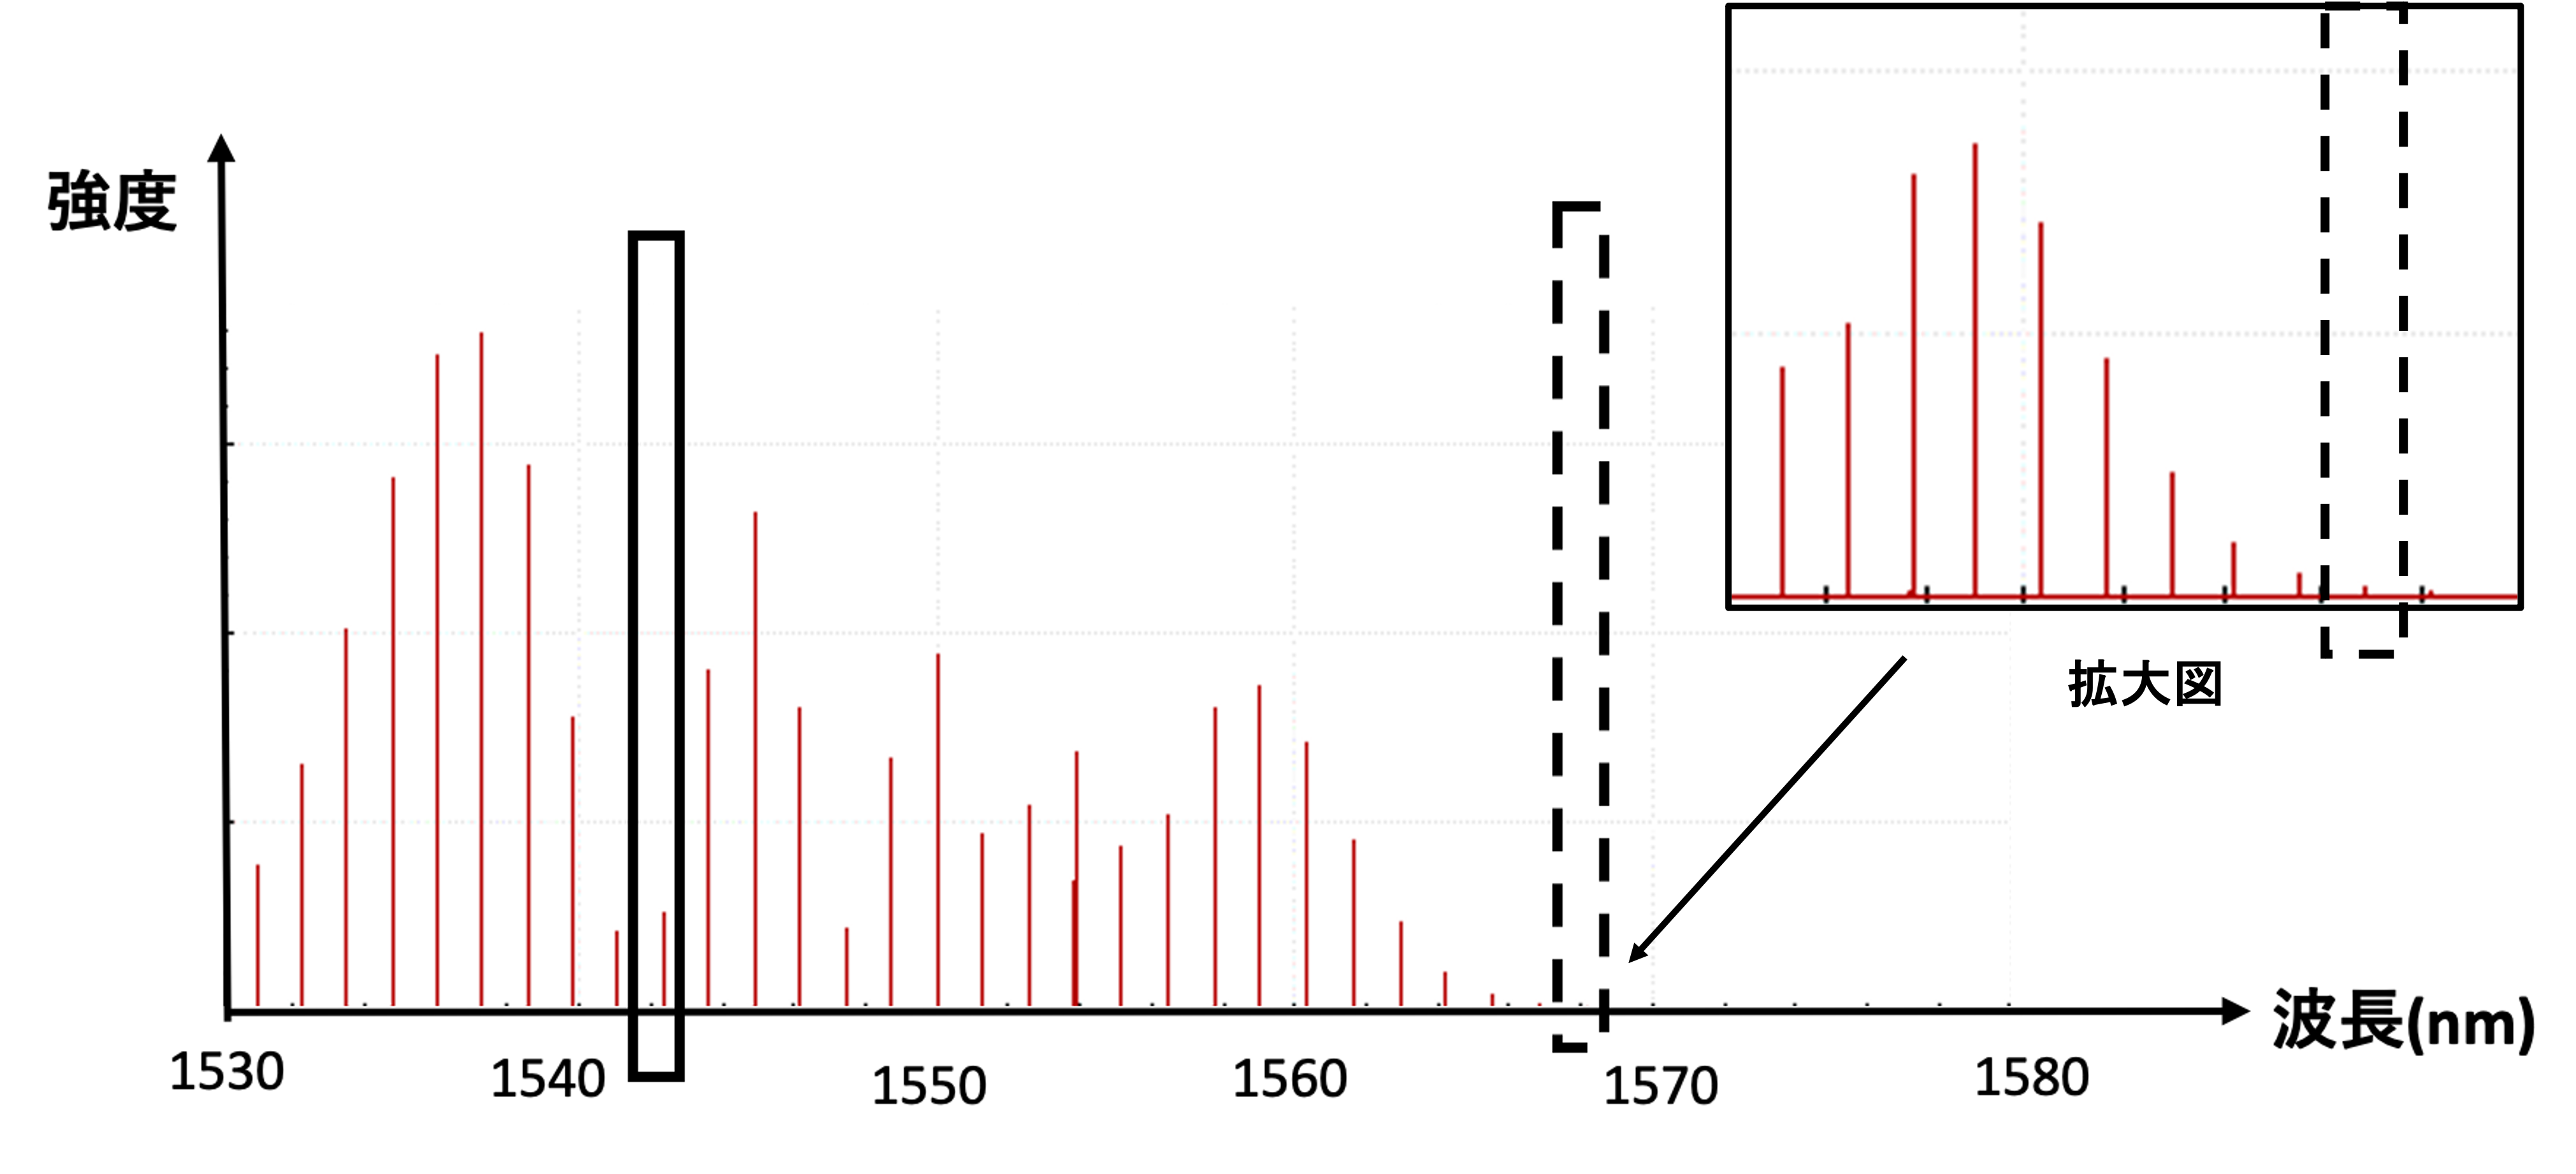
\includegraphics[width=7cm]{images/11_spectrum.png}
      \caption{入力光A=1, 入力光B=1の場合のスペクトラム}
    \end{minipage}
  \end{tabular}
\end{figure}

\begin{itemize}
  \item 入力光が互いに0の場合 \\
  QD-SOA内で非線形光学効果が発生せず制御光が大きく増幅される.
  \item 入力光のどちらかのみが1の場合 \\
  QD-SOA内で非線形光学効果であるXGMによって入力光に利得が奪われるため制御光があまり増幅されない.
  さらにXPMによってスペクトルが広がる.
  \item 入力光が互いに1の場合 \\
  XGMによって制御光はほとんど増幅されない.
  さらにXPMによってスペクトルが大きく広がる
\end{itemize}

\subsection{シミュレーション結果}
注入電流を 300mA に固定し, `1'強度を -20dBm から 10dBm の範囲で変化させると
図5に見られるように,最もお互いの消光比の値が大きい入力光強度は10dBmとなった.\\
AND演算およびXOR演算を行った場合のシミュレーション結果をアイダイアグラムの形で描画すると図6,7のように表せる.
AND演算における消光比は14.89dB, XOR演算における消光比は10.21dBが得られた.
\begin{figure}[H]
  \centering
  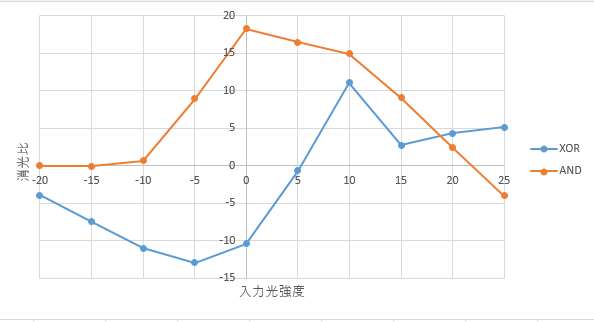
\includegraphics[width=11cm]{images/input_er.png}
  \caption{入力光強度による消光比の推移}
\end{figure}
\begin{figure}[H]
  \begin{tabular}{cc}
    \begin{minipage}[t]{0.45\hsize}
      \centering
      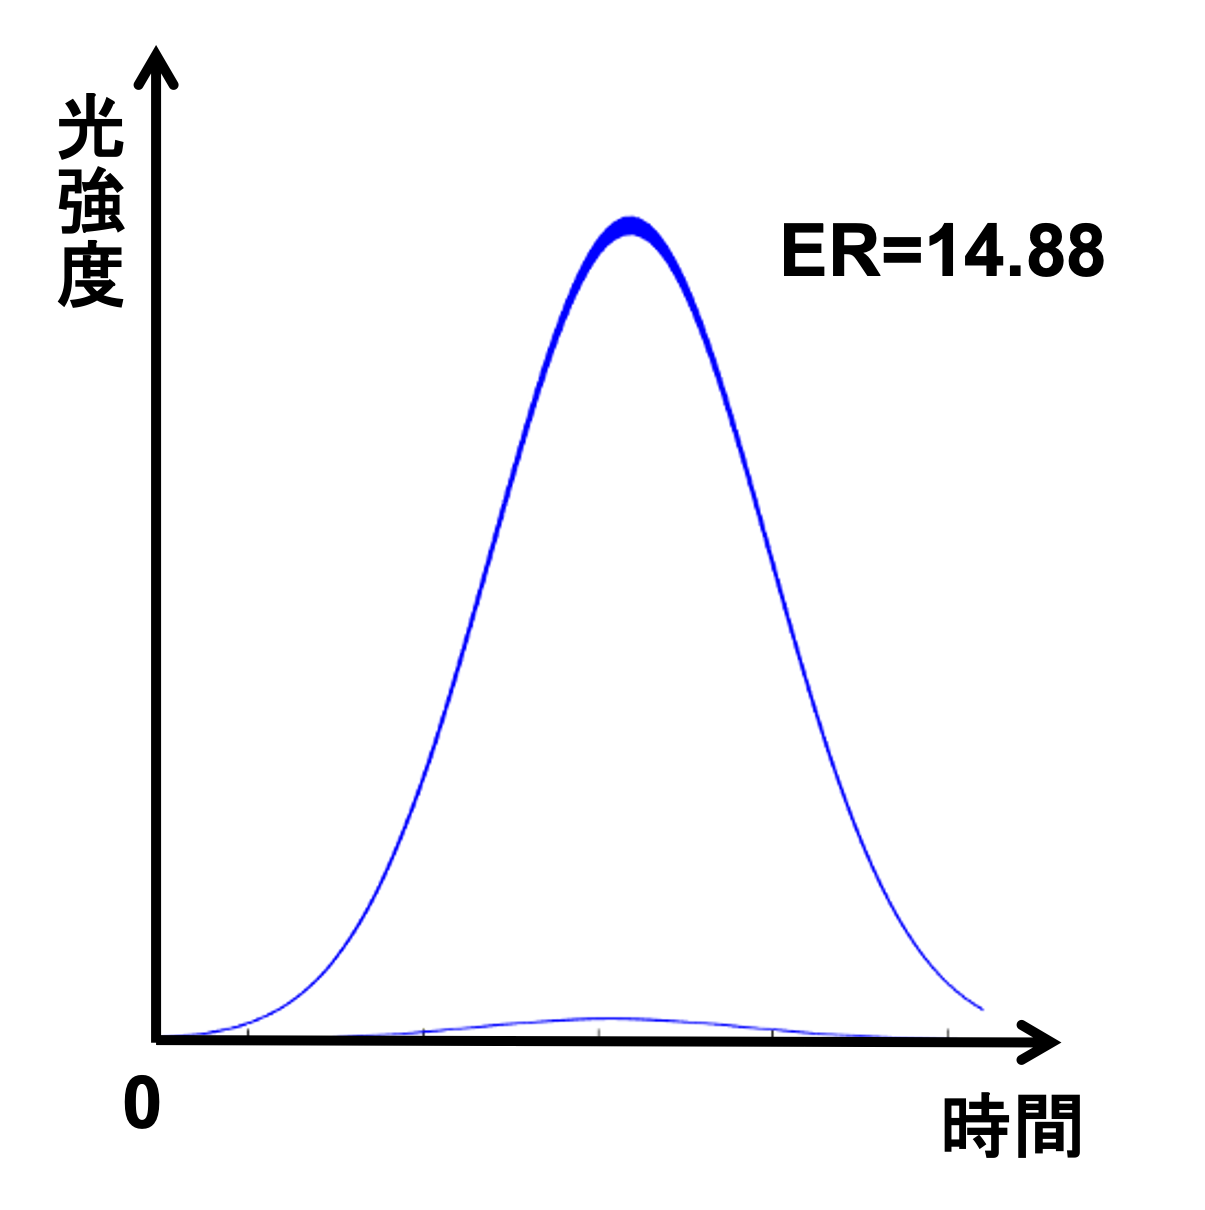
\includegraphics[width=7cm]{images/and_result.png}
      \caption{AND回路の結果}
    \end{minipage} &
    \begin{minipage}[t]{0.45\hsize}
      \centering
      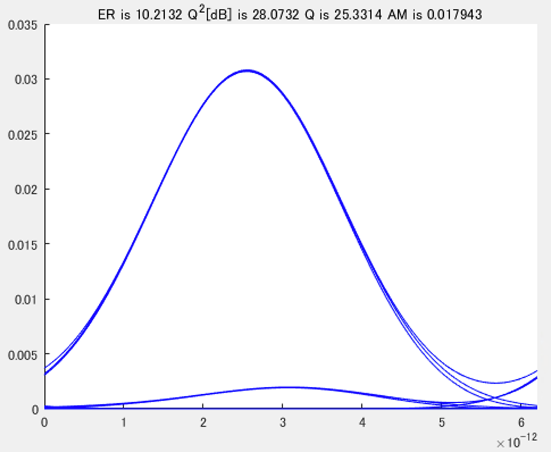
\includegraphics[width=7cm]{images/xor_result.png}
      \caption{XOR回路の結果}
    \end{minipage}
  \end{tabular}
\end{figure}

\section{まとめ}
単一QD-SOAを用いた全光AND/XOR論理回路を提案した.
シミュレーション結果より論理回路の動作を確認でき, 評価指標から出力波形の品質は良好と見られる.

\begin{thebibliography} {99}
  \bibitem{singleXORゲート} E.Dimitriadou and K.E.Zoiros, “All-Optical XOR Gate Using Single Quantum-Dot SOA and Optical Filter”, Journal of lightwave Technology, vol.31, NO.23, Dec. 2013.
  \bibitem{参照ラベル2名} K.Komatsu et al, “All-optical NOR gate using a single quantum-dot SOA-assisted an optical filter,“ Opt, Quant. Electron., vol. 50, no. 3, pp. 1-18, Feb 2018.
\end{thebibliography}

\end{document}
